\section{Métodos}

Boscá et. al. \cite{Bosca15} mencionan que existe una similitud entre FHIR y enfoques como el utilizado en openEHR. Dado que los recursos de FHIR y los arquetipos de openEHR definen patrones reutilizables para la descripción precisa de la información clínica. Sin embargo, los trabajos de colaboración entre las comunidades de FHIR y openEHR \cite{Collaboration} no consiguieron relacionar recursos y arquetipos existentes que representan conceptos clínicos similares debido a los principios de diseño diferentes utilizados por ambas comunidades. Siendo la principal diferencia que los arquetipos esperan representar la mayoría del contenido clínico, mientras que los recursos solo contienen la información clínica utilizada más común.

Sin embargo, como un recurso FHIR contiene un conjunto de elementos de datos estructurados descriptos en la definición de su tipo \cite{FHIRResource}, y un arquetipo openEHR constituye una encapsulación de un conjunto de puntos de datos pertencientes a un contenido de dominio, expresado en términos de restricciones del modelo de información de referencia openEHR \cite{openEHRArchetype}, una forma de encontrar correspondencia entre un recurso FHIR y un arquetipo openEHR es encontrar las relaciones entre los elementos de datos del recurso FHIR y los puntos de datos del arquetipo openEHR. El enfoque propuesto en este trabajo para encontrar estas relaciones es crear un nuevo arquetipo openEHR a partir de la definición de un recurso FHIR existente.

Debido a que la definición de un elemento en un recurso FHIR incluye tipo de dato \cite{FHIRElement}, es un prerrequisito encontrar las equivalencias entre los tipos de datos FHIR y los tipos de datos openEHR.

La creación de un arquetipo openEHR a partir de la definición de un recurso FHIR utilizando las equivalencias de tipos de datos puede ser sencilla. Dentro de un editor de arquetipos como los citados en \cite{openEHRModellingTools}, se puede crear de forma manual el arquetipo openEHR modelando la misma estructura del recurso FHIR utilizando el tipo de dato openEHR donde corresponda teniendo en cuenta las equivalencias de tipos de datos. Una alternativa diferente se presenta en este trabajo, consistente en la creación a través de un proceso automatizado. Las ventajas de esta alternativa frente al tipo de creación manual son un tiempo de creación y un riesgo de introducir errores por factor humano menores.

\begin{figure*}[t]
  \centering
  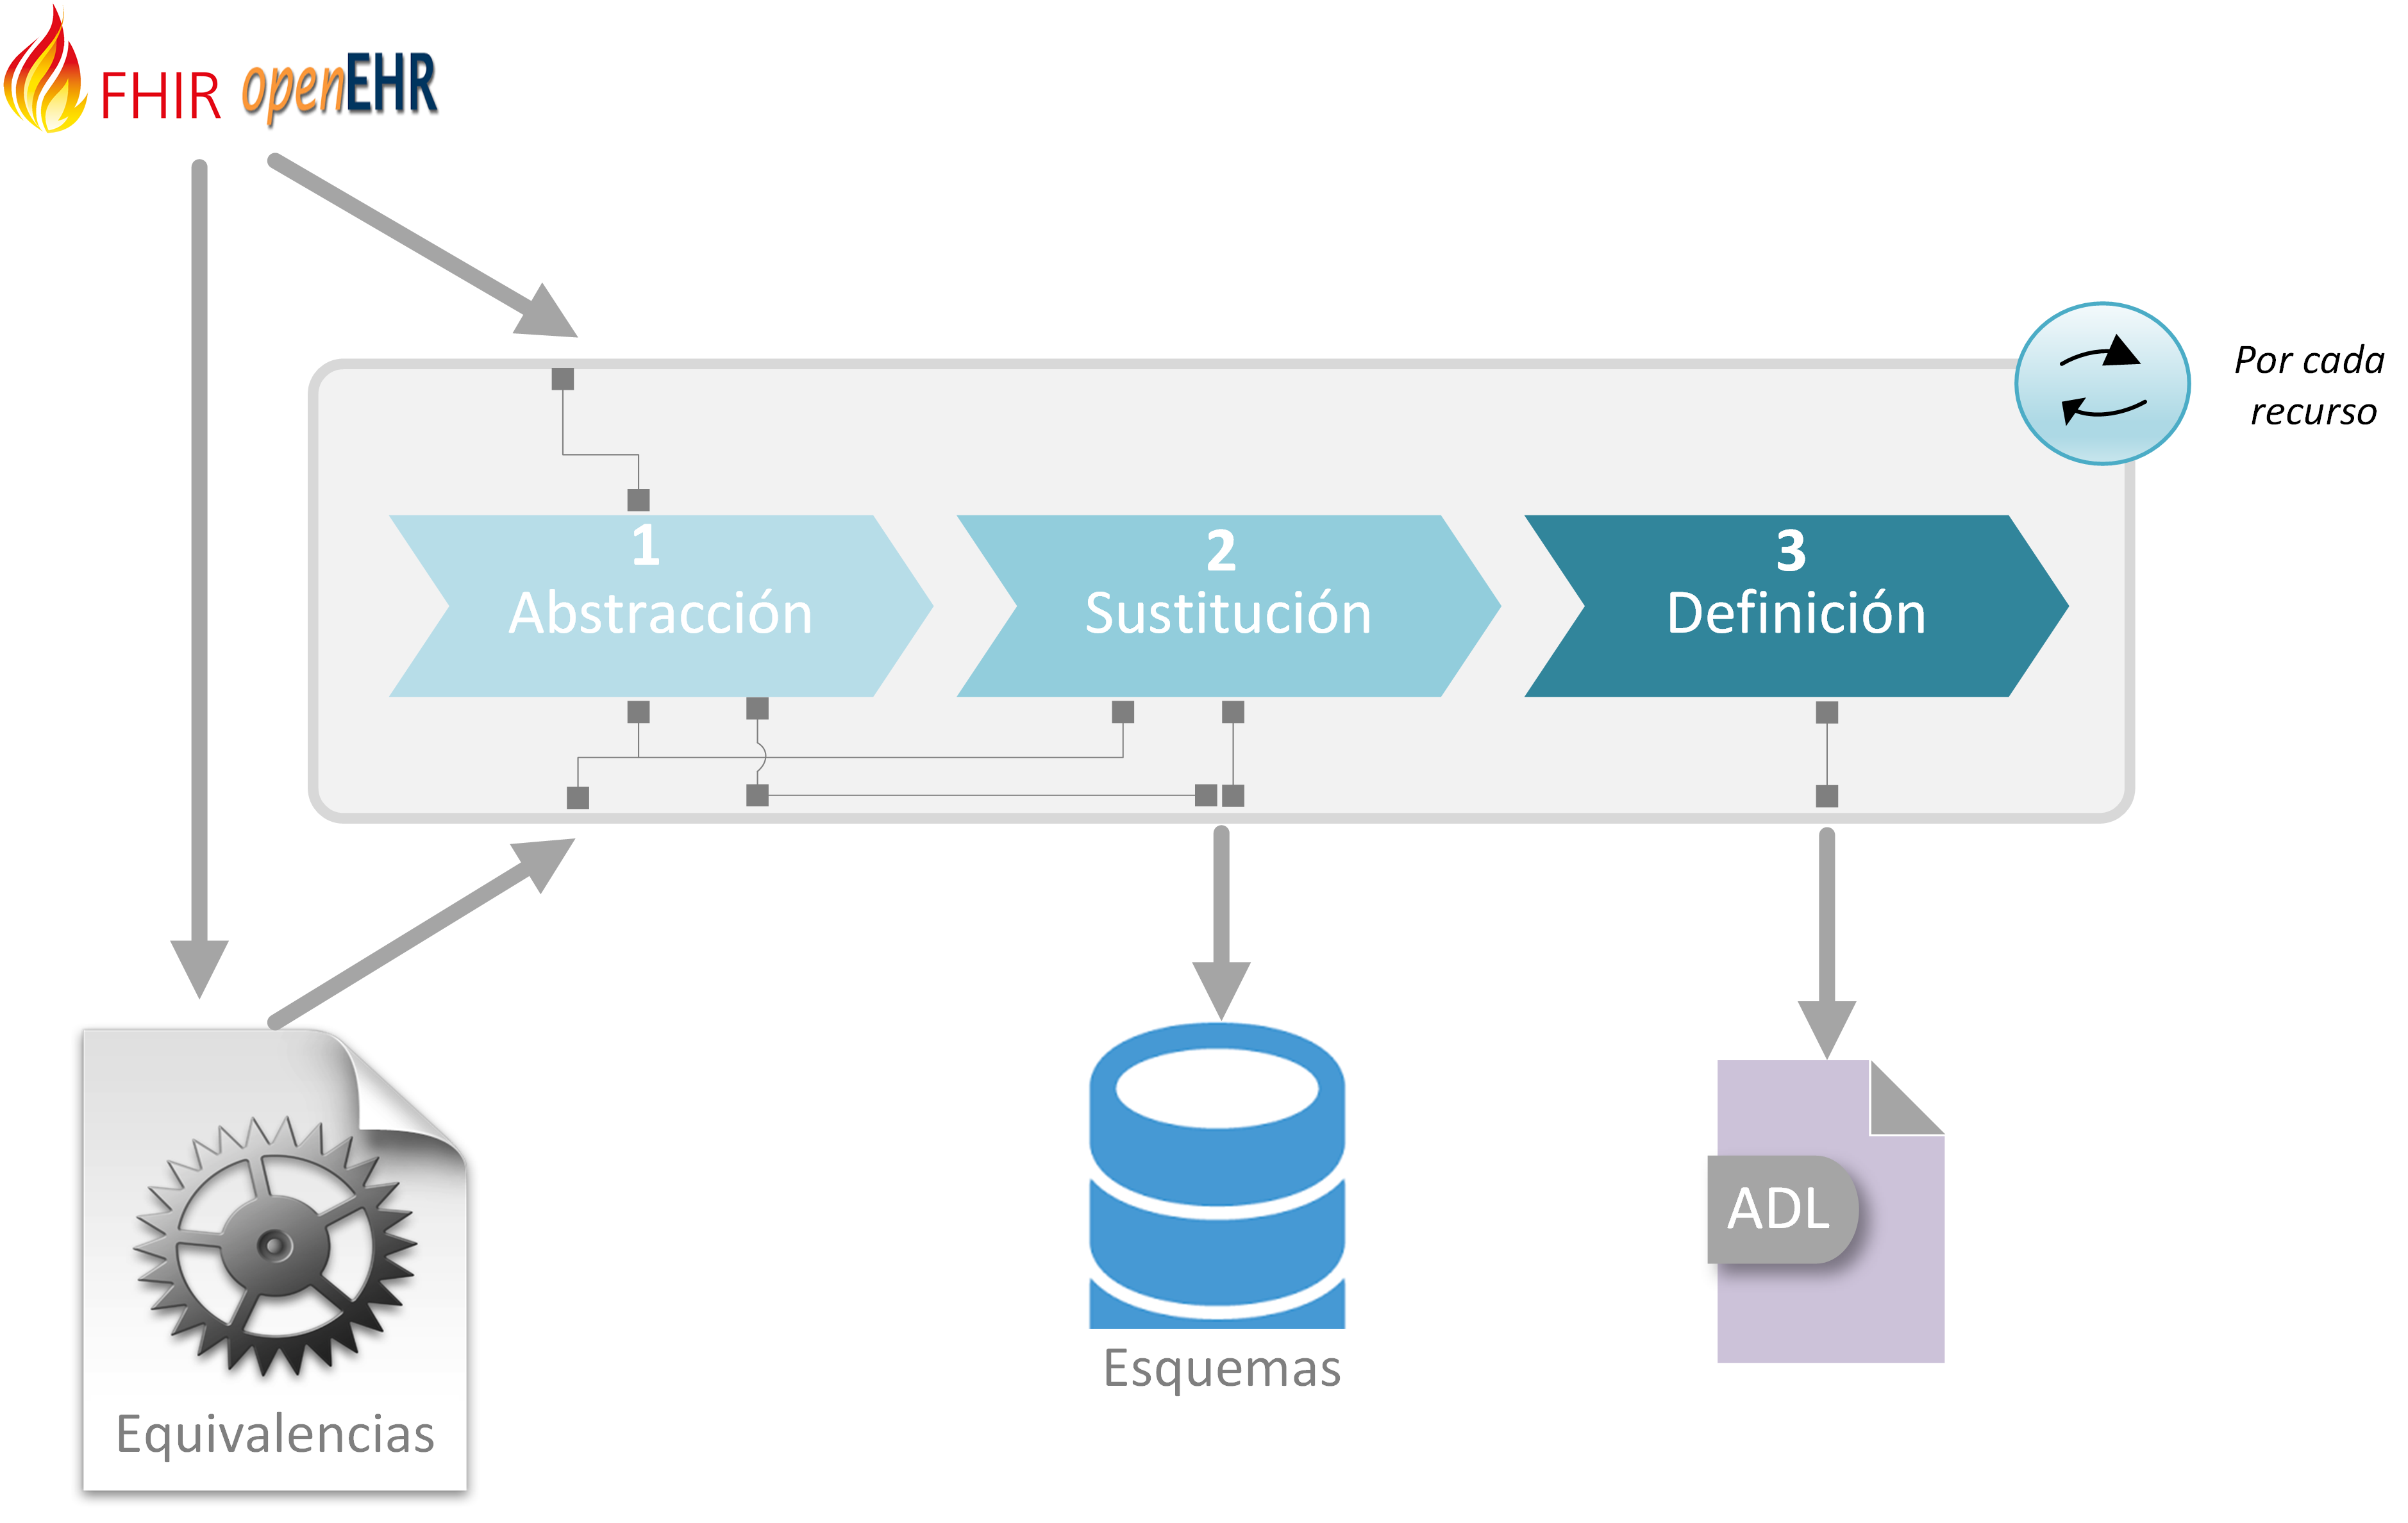
\includegraphics[scale=0.6]{./images/solution}
  \caption{Proceso automatizado}
  \label{fig:solution}
\end{figure*}

\subsection{Equivalencias entre tipos de datos}

Una equivalencia entre un tipo de dato primitivo de FHIR y un tipo de dato de openEHR existe si se cumplen las condiciones de:

\begin{enumerate}
  \item el dominio de valores del tipo de dato de FHIR puede ser almacenado dentro de uno de los atributos del tipo de dato de openEHR;
  \item el uso del tipo de dato de openEHR para el cual fue diseñado se conserva.
\end{enumerate}

Como un ejemplo, el tipo de FHIR boolean y el tipo de openEHR DV\_BOOLEAN reúnen ambas condiciones, por lo tanto, son equivalentes:
\begin{enumerate}
  \item los valores true y false del dominio de valores del tipo boolean pueden ser almacenados dentro del atributo value del tipo DV\_BOOLEAN;
  \item el uso de DV\_BOOLEAN, el cual especifica que el tipo se usa para elementos que son datos verdaderamente booleanos, se conserva.
\end{enumerate}


\subsection{Automatización}

Con el fin de comparar los tiempos de creación manual y automática, se llevó a cabo un experimento en el cual se comparó el tiempo requerido para la creación manual y automática del arquetipo de openEHR de recurso Flag de FHIR. Para la creación manual se utilizó el editor ADL WORKbench \cite{ADLWORKbench}. Para la creación automática se implementó el proceso (ver Figura 1) en el lenguaje Python, el cual retorna arquetipos con estructuras equivalentes a los recursos. Los resultados del experimento (ver Cuadro \ref{table:automation}) muestran una reducción significativa en el tiempo de creación usando el proceso automático.

\begin{table}
  \caption{Automatización}
  \label{table:automation}
  \begin{tabular}{l l}
    \hline
    Creación Manual	& Creación Automática \\
    \hline
    Aprox. 30 minutos	& Aprox. 180 milisegundos \\
    \hline
  \end{tabular}
\end{table}

